\documentclass{article}

% if you need to pass options to natbib, use, e.g.:
%     \PassOptionsToPackage{numbers, compress}{natbib}
% before loading milestone

% ready for submission
% \usepackage{milestone}

% to compile a preprint version, e.g., for submission to arXiv, add add the
% [preprint] option:
%     \usepackage[preprint]{milestone}

% to compile a camera-ready version, add the [final] option, e.g.:
     \usepackage[final]{milestone}
    
% to avoid loading the natbib package, add option nonatbib:
%     \usepackage[nonatbib]{milestone}

\usepackage[utf8]{inputenc} % allow utf-8 input
\usepackage[T1]{fontenc}    % use 8-bit T1 fonts
\usepackage{hyperref}       % hyperlinks
\usepackage{url}            % simple URL typesetting
\usepackage{booktabs}       % professional-quality tables
\usepackage{amsfonts}       % blackboard math symbols
\usepackage{nicefrac}       % compact symbols for 1/2, etc.
\usepackage{microtype}      % microtypography
\usepackage{graphicx}
\graphicspath{ {./images/} }
\title{Flappy Bird using Q-Learning}

% The \author macro works with any number of authors. There are two commands
% used to separate the names and addresses of multiple authors: \And and \AND.
%
% Using \And between authors leaves it to LaTeX to determine where to break the
% lines. Using \AND forces a line break at that point. So, if LaTeX puts 3 of 4
% authors names on the first line, and the last on the second line, try using
% \AND instead of \And before the third author name.

\author{%
  Jesse A. Pelzar\\
  Department of Electrical and Computer Engineering\\
  Binghamton University\\
  Binghamton, NY 13850\\
  \texttt{jpelzar1@binghamton.edu} \\
  \url{https://jessepelzar.github.io/Flappy_Bird_RL/}
  % examples of more authors
  % \And
  % Coauthor \\
  % Affiliation \\
  % Address \\
  % \texttt{email} \\
  % \AND
  % Coauthor \\
  % Affiliation \\
  % Address \\
  % \texttt{email} \\
  % \And
  % Coauthor \\
  % Affiliation \\
  % Address \\
  % \texttt{email} \\
  % \And
  % Coauthor \\
  % Affiliation \\e
  % Address \\
  % \texttt{email} \\
}

\begin{document}

\maketitle


\section{Introduction}


This project is based off of the well known mobile game Flappy Bird. With my strong background in web based technologies, I decided to recreate the game Flappy Bird within a web environment with the ability to not only play Flappy Bird, but the ability to have the the agent (the bird) learn how to avoid hitting the moving obstacles, floor or ceiling. The Reinforcement Learning component to this game was Q-Learning which allows the agent to learn through exploration and exploitation by optimizing the best action to take when in a given state. With a constantly changing environment, the agent must adapt to updated positioning of obstacles in order to avoid them. The importance of this project is to learn and adapt to a constantly changing environment while utilizing similarities such as comparing distances to achieve a different reward. The methods I incorporated are interesting and have the ability to be applied to other environments that may resemble a similar concept but consist of different states and actions.  

\section{approach}

When considering the implementation of Reinforcement Learning, it's important to  determine what will make up the environment. this includes the actions, states, rewards and other variable such as a discount factor and exploration probability. Using Q-Learning, I was able to implement a model free learning approach that derives an optimal policy using time difference learning to constantly update the Q table values on each iteration. 

\subsection{Choosing Actions}

In the game Flappy Bird, the bird is locked in x-space but has free range in the y-space. The actions capable by the bird are either jump or not jump. When the birds action is not jump, it will fall down to the ground, which loses the game. On the project website, you will have the ability to configure the type of jump that the agent can perform. The Standard jump mode is an arching jump that accelerates and decelerates, similar to the original game. The Linear jump mode has two variables that represent static jumping and falling velocities. In this project, the bird which represents the agent, must choose what states require a jump and which ones don't. 

\subsection{Determining Environment States}

\begin{figure}[h]
    \centering
    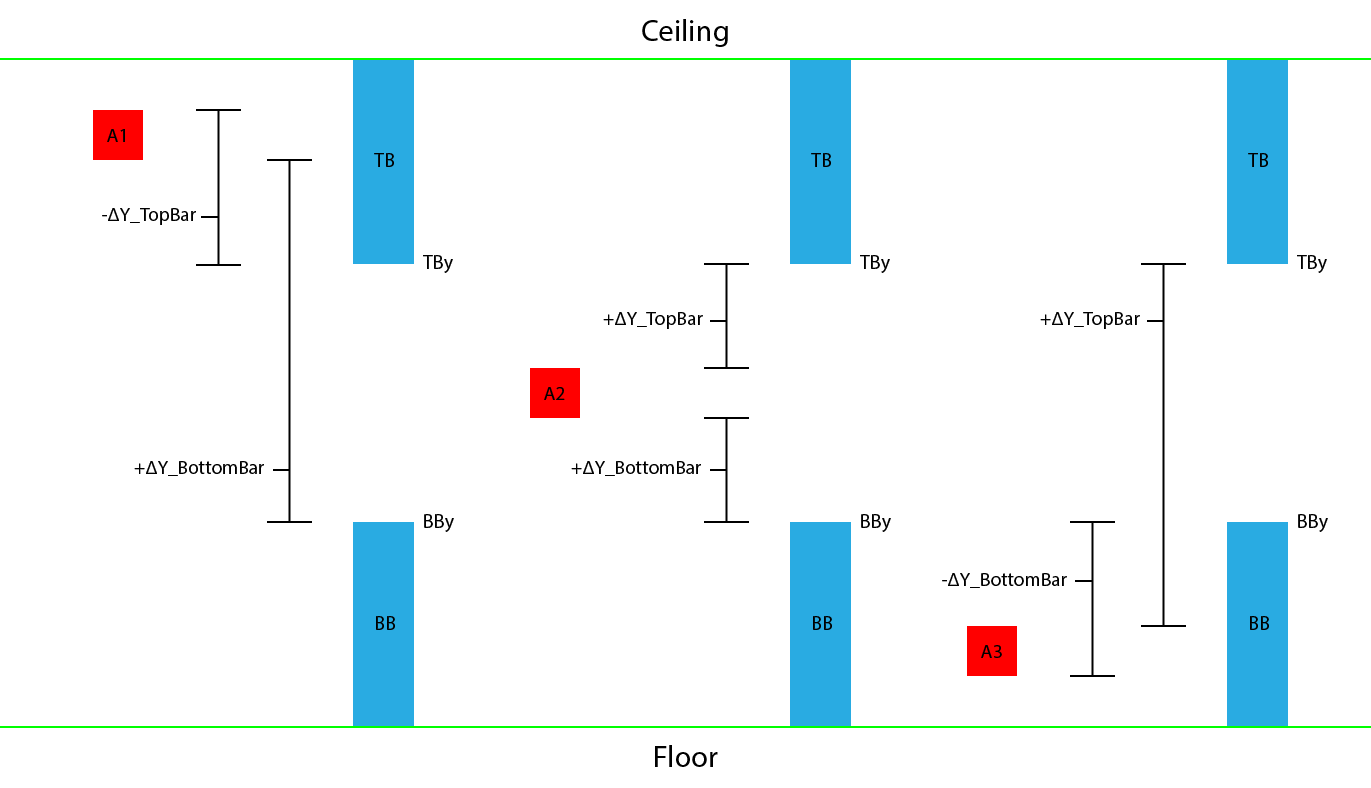
\includegraphics[width=0.75\textwidth]{figure0}
    \caption{Vertical Differencest}
    \label{fig:mesh1}
\end{figure}



In order for the agent to know its position in the environment, the agent must always be located in a state (s) which is a member of a discrete number of states in a set (S). States can be represented in a variety of ways including positioning in an environment, location relationships of obstacles, or even a combination of the two. In my development, I decided to represent the states by utilize the characteristics of the moving obstacles within the environment. These obstacles are referred to as the top bar, represented as TB and the bottom bar represented as BB, where TB is on the ceiling while BB is positioned directly below but on the floor. 



\subsection{Vertical difference between agent height and obstacles}

When considering the states, rather than only using a single variable to represent the current state of the agent, the method I developed utilizes two variables. The first variable is derived from the vertical difference between top of the agent's height and the vertical position of TB's lowest part (TBy),  whereas the second variable is derived from the vertical difference between the bottom of the agent's height and the vertical position of BB's highest part (BBy).

Represented in figure 1, the agent is shown in three different positions, A1, A2, and A3. In position A1, the vertical difference between the top of the agent to the TBy scales negatively where as the vertical difference between the bottom of the agent to the BBy scales positively. With position A3 the vertical differences are the opposite of A1's with the vertical difference between the top of the agent to the TBy scales positively where as the vertical difference between the bottom of the agent to the BBy scales negatively. Last the position of A2 shows both of the vertical differences remaining positive. 


\begin{figure}[h!]
    \centering
    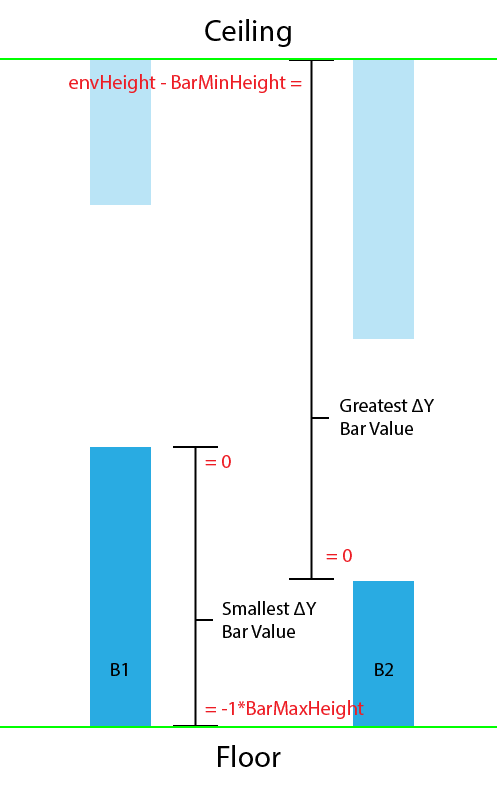
\includegraphics[width=0.5\textwidth]{figure2}
    \caption{Largest range of vertical distance values}
    \label{fig:mesh2}
\end{figure}

\subsection{Mapping to state indexes}



In order to know the true range of vertical difference from the smallest negative value to the largest positive value, it's important to know the maximum height of an obstacle as well as the minimum height. This tells us that the lowest value the state can be is the length of the tallest obstacle multiplied by negative 1 and that the greatest value the state can be is the height of the shortest obstacle subtracted from the height of the environment, in this case the game canvas. This is visually represented in figure 2. Gathering the values from the vertical differences for the purpose of representing states means that when indexing the Q table, all of the indexes must be positive. When running, these values are stored as class variables that are passed as arguments to a function that maps them to positive integers. The mapping of the values also grants the ability to choose the range from zero to the number of desired states represented in figure 3. This variable is modifiable on the project webpage. 

\begin{figure}[h!]
    \centering
    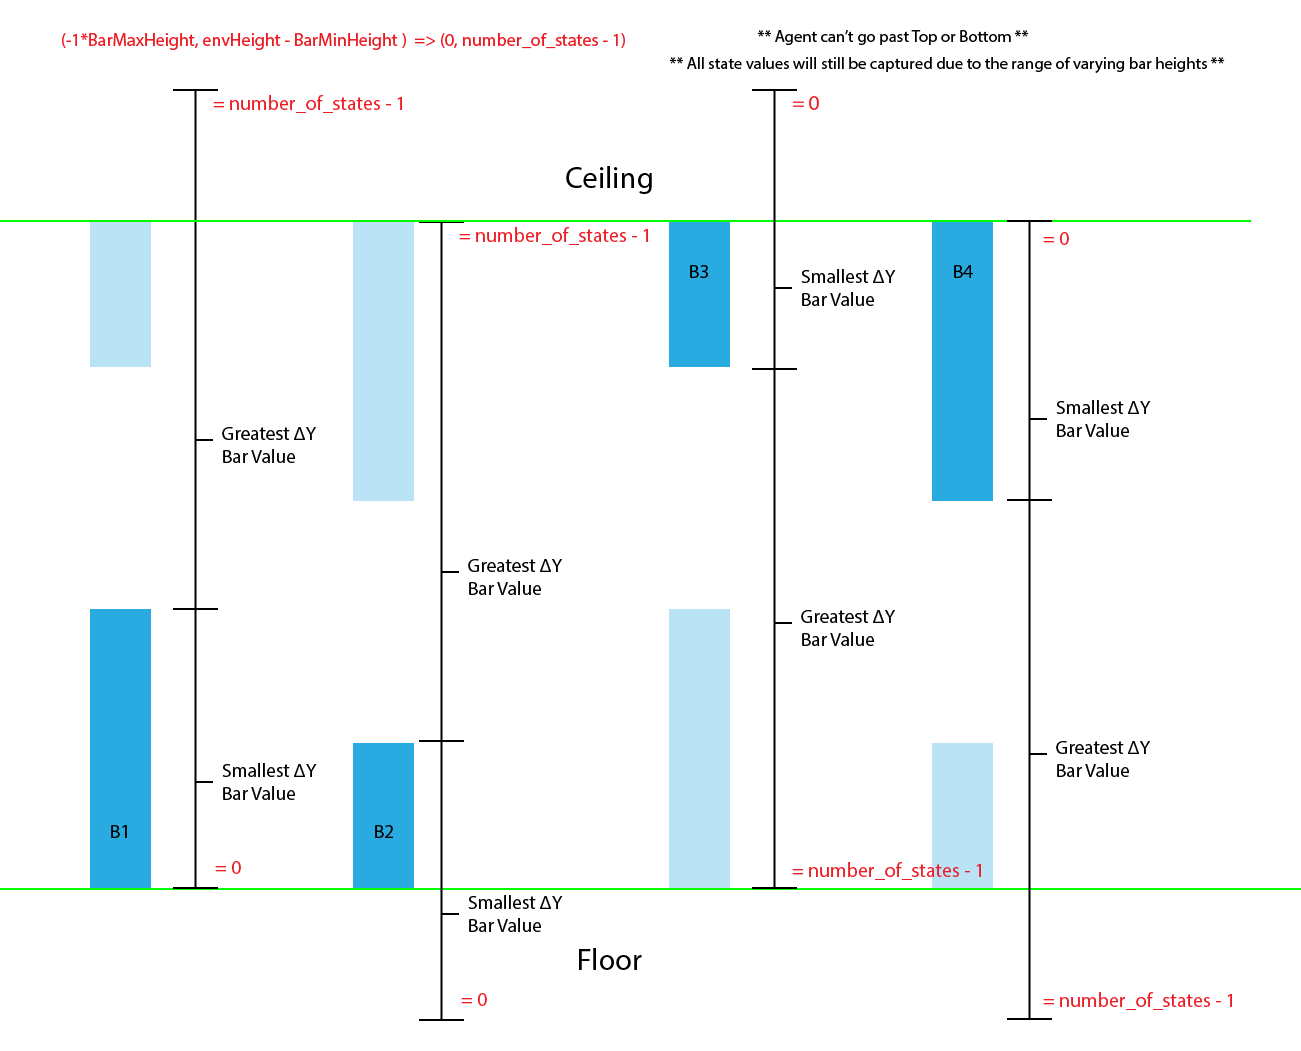
\includegraphics[width=1\textwidth]{figure3}
    \caption{Largest range of vertical distance values mapped}
    \label{fig:mesh2}
\end{figure}

\subsection{Rewards}

\begin{figure}[h!]
    \centering
    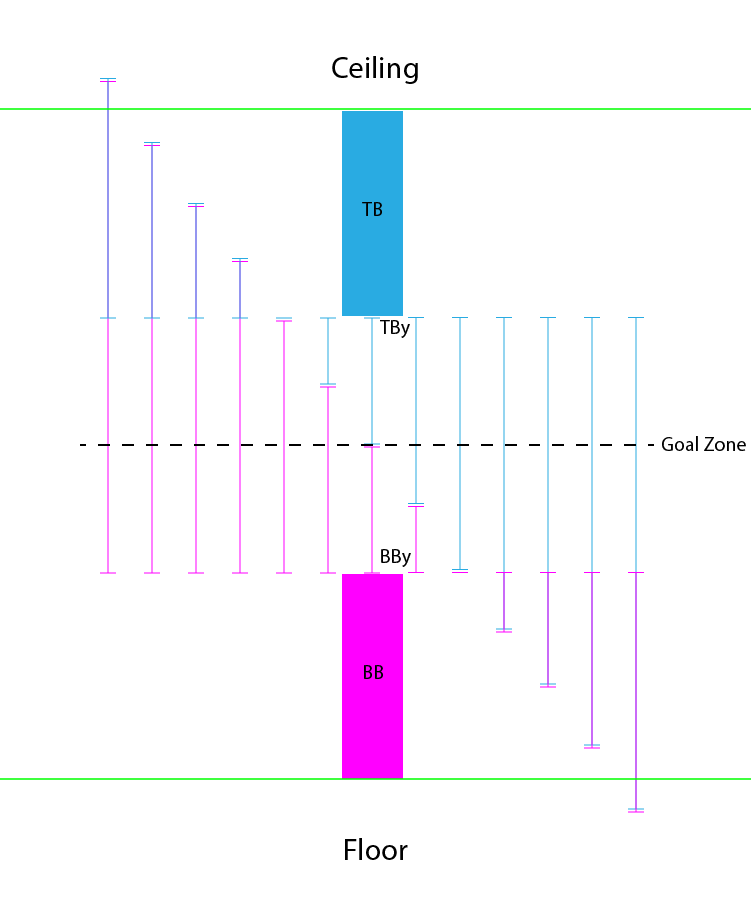
\includegraphics[width=1\textwidth]{figure4}
    \caption{Example of reward zones}
    \label{fig:mesh2}
\end{figure}

Rewards are necessary for telling the agent if a chosen action for a set of states is the best action to take. Utilizing the vertical difference algorithm to do this reduces the need for additional processes and is overall more efficient. Because the objective of the agent is to make it through the gap between the obstacles, veering away from this goal zone must issue a penalty or negative reward. The method I came up with is shown in figure 4 and mathematically represented in the equation below. Taking the absolute value of the difference between TBy and BBy and raising it to a power of some value will exponentially increase as the difference becomes larger. When multiplied by negative one, the reward value decreases exponentially by the power it was raised too. With an exponentially decreasing reward, the further the agent moves from the goal zone, the larger the penalty will be.
\begin{equation}
Reward = (|TBy-BBy|^{x}) * -1
\end{equation}

\subsection{Results}
The results showed success with all tests and is fully working to try out in the link on the first page.




%
%
%\section*{References}
%
%References follow the acknowledgments. Use unnumbered first-level heading for
%the references. Any choice of citation style is acceptable as long as you are
%consistent. It is permissible to reduce the font size to \verb+small+ (9 point)
%when listing the references. {\bf Remember that you can use more than eight
%pages as long as the additional pages contain \emph{only} cited references.}
%\medskip
%
%\small
%
%[1] Alexander, J.A.\ \& Mozer, M.C.\ (1995) Template-based algorithms for
%connectionist rule extraction. In G.\ Tesauro, D.S.\ Touretzky and T.K.\ Leen
%(eds.), {\it Advances in Neural Information Processing Systems 7},
%pp.\ 609--616. Cambridge, MA: MIT Press.
%
%[2] Bower, J.M.\ \& Beeman, D.\ (1995) {\it The Book of GENESIS: Exploring
%Realistic Neural Models with the GEneral NEural SImulation System.}  New York:
%TELOS/Springer--Verlag.
%
%[3] Hasselmo, M.E., Schnell, E.\ \& Barkai, E.\ (1995) Dynamics of learning and
%recall at excitatory recurrent synapses and cholinergic modulation in rat
%hippocampal region CA3. {\it Journal of Neuroscience} {\bf 15}(7):5249-5262.
%
\end{document}